\documentclass[fleqn]{article}
\usepackage[export]{adjustbox}
\usepackage{wrapfig, lipsum}
\usepackage{xcolor}
\usepackage{listings}
\usepackage{float}
\usepackage{graphicx}
\usepackage{amsmath}
\usepackage{amssymb}
\usepackage{amsfonts}
\usepackage{amsthm}
\usepackage{geometry}
\usepackage{booktabs}
\usepackage{etoolbox}
\usepackage{algorithm}
\usepackage{algpseudocode}
\usepackage{subfig}



\algtext*{EndIf}% Remove \EndIf

\newcommand{\white}[3] {
  \foreach \x in {0, ..., #3} {
    \draw[fill=white] ({.5+#1},{\x*.1+.5+#2}) circle (0.42) node {#3};
  }
}
\newcommand{\black}[3] {
  \foreach \x in {0, ..., #3} {
    \draw[fill=white!70!black] ({.5+#1},{\x*.1+.5+#2}) circle (0.42) node {#3};
  }
}
\newcommand{\colorSquare}[3] {
  \draw[fill=#1] ({#2},{#3}) rectangle ({#2+1},{#3+1});
}

 \geometry{
 a4paper,
 total={170mm,257mm},
 left=20mm,
 top=20mm, 
 bottom=15mm,
 }


\title{\vspace{-20mm}COMP30023 Artificial Intelligence Project part-a Report}
\author{William Lord and Luke Hawkins}

\begin{document}
\maketitle
\section{Formulation of game as search problem:}
	 The \textit{board state} (game state) is a Board class instance containing a dictionary of pieces, with the key as an $(x,y)$ tuple corresponding to the position, and the value, a Tile class instance whose containing the owner of the token and stack size. If a position is not a key in the dictionary, then the position is unoccupied. The board state can only be modified by applying one of two operations to the current state:  a \text{move} action or a \text{boom} action.\\

	 \noindent A \text{move} operation allows the player to move their pieces from one position on the board to another position on the board. In this regard, a move is a permutation of the board state.\\
	 
	 \noindent A \textit{boom} operation allows a player to explode one of their pieces at its current position on the board, which also exploding any other pieces within 1 chebyshev distance recursively. A boom reduces positions occupied in the board state, lowering complexity.\\
	 
	 \noindent Our target goal state is for there to be no enemy pieces and zero or more of our own. A failed state is when we have no pieces left and the enemy still has pieces remaining. A solution is a sequence of operations to reach the goal state, with each operation incurring a unit 1 cost.

\section{Search algorithms used and why:}
	Our algorithm combines breadth first search (\textit{bfs}) and depth first search (\textit{dfs}). Our algorithm runs bfs and expands nodes until we encounter a boom action that is within 1 chebyshev distance of an enemy token, once a boom action is processed  our algorithm recurses on the new board state post recursive explosions. Hence we bfs to find the next boom action, and dfs between boom actions. See Figure 1(b).\\

\noindent The algorithm implicitly uses the heuristic that boom actions reduce the path cost to the goal state more than a move does (which is why we immediately recurse on boom actions close to enemy tokens), as any boom action reduces the number of enemy pieces on the board and thus the complexity of the board, and greedily expands boom actions via dfs. For reasons below our algorithm is not optimal, hence our heuristic cannot be admissible (or consistent).\\
	
	\noindent We settled upon our algorithm because it is complete, and although it sacrifices the optimality bfs provides, practically, it is faster due to our heuristic.\\
	
	\noindent \underline{Completeness}: Our algorithm is complete. As at one level it is bfs which is always complete and at dfs which is complete for finite depth, the max depth (number of booms in this context) is the same as the number of our tokens, at most 3.\\
	
	\noindent \underline{Optimality}: Our algorithm is not optimal due to the dfs component, as dfs is inherently non-optimal. However between each boom it will find an optimal path to that boom action which can lead to a goal state, as this is using bfs (the boom action it finds may nto be part of the overall shortest path though, the source of non-optimality). If we only have 1 token, then our algorithm is optimal (since it is just vanilla bfs).
	 \begin{enumerate}
		\item $m$\textit, maximum depth of the tree;
	 	\item $m_{dfs}$\textit, maximum depth of dfs action;
		\item $d_{bfs}$\textit, optimal path depth to a boom in a winning sequence (this is different than vanilla bfs' $d$);
	 	\item b\textit, branching factor (moves and boom).

	 \end{enumerate}
	
	\noindent \underline{Time Complexity}: Our time complexity is $O(b^m)$. Since our algorithm is non-optimal, we may terminate at the maximum depth.\\
	
	\noindent \underline{Space Complexity}: Our space complexity is a little complicated. The bfs component stores every level until a solution, thus $bfs = O(b^{d_{bfs}})$ and the dfs component only stores current and parent levels, each level is a bfs, thus $dfs = O(m_{dfs}bfs))$. Thus overall $O(m_{dfs}(b^{d_{bfs}})).$\\

\begin{figure}%
   \centering
  	\subfloat[Snaking example]{{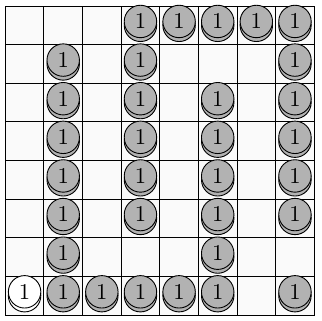
\includegraphics[width=7.3cm]{snaking} }}%
   	\qquad
    	\subfloat[Algorithm Visualisation]{{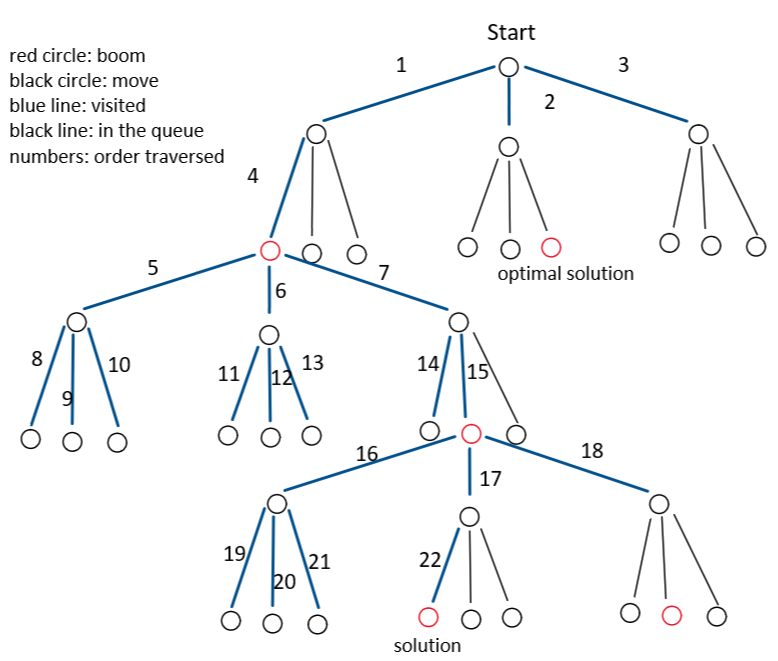
\includegraphics[width=7.3cm]{algorithm_explanation} }}%
	  \label{fig:example}%
\end{figure}
\section{Time and space requirements:}

\noindent The time and space complexity for our algorithm is a function of the branching factor $b$ and the maximum depth of the tree $m$. $b$ is heavily influenced by the moves available. The inputs provides that the player will only receive a maximum of three pieces to start with. This directly effects the maximum value for $b$. Further $m$ is influenced by how many booms can be taken and how many moves to explore a given board state.\\

\noindent For any given piece, $b$ has an upper bound of $4k^2 + 1$ moves available, where $k$ is the pieces' stack size. The constant factor 4 is the number of cardinal directions the piece could move in and the $+1$ is the boom move available. Since $k$ is capped at 3 by the inputs, theoretically, the highest $b$ could be is $37$ moves for a given state.\\

\noindent $m$ is the product of the max amount of booms available, $m_{dfs}$ at most $k$, and how deep each bfs is, $d_{bfs}$, and is a function of $L$ the length of the board, in our case $L=8$. An approximate upper bound for $d_{bfs}$ would be where the token has to snake through paths of black tokens, going up and then back down, which has $O(L^2)$ complexity (See Figure 1(a)). Hence $O(m) = O(kd_{bfs}) = O(kL^2).$\\

\noindent \underline{Time Complexity}: Combining these results we see that our algorithm has a time complexity of $O({bfs} {dfs})= O(b^m) =  O((4k^2+1)^{kL^2})$, where $b = 4k^2 + 1$ and $m=  kL^2$.\\

\noindent Increasing $k$ increases the amount of depth for dfs, and increasing the board length increases the depth for bfs quadratically in $L$, overall increasing the maximum depth. Similarly, decreasing $k$ decreases the maximum depth. Furthermore, since each boom reduces $k$ by at least 1, although our algorithm runs in $O(b^m)$ time, we reduce both $b$ and $m$ every boom (per above) quadratically in $k$ thereby giving us a practicable running time. On the flipside, increasing the board size ($L$), or the amount of initial tokens ($k$), would have an exponential effect on the practical running time of our algorithm. \\

\noindent \underline{Space Complexity}: Our space complexity above is $O(m_{dfs}(b^{d_{bfs}}))$. Per above, we have $b = 4k^2 + 1$, $O(d_{bfs}) = L^2$ and $m_{dfs} = k$. Hence, our space complexity becomes $O(k(4k^2+1)^{L^2})$.\\

\noindent The space complexity scales in a somewhat similar way. Each bfs will contain considerably less space then its parent, from the quadratic nature of the branching factor, and then store at most k of these bfs'. While the increase in board width, L, has an exponential effect from causing an increase in the depth of the bfs. \\

\noindent The positioning of the black tokens only really effects the $d_{bfs}$ by blocking the tokens path to maneuvare to a correct position. However, short of pathological cases, eg Figure 1(a), this in general would only increase the depth of the bfs by 1 or 2.


\end{document}